\chapter{Wyniki eksperymentalne}

Aby podsumować dotychczas omówione zagadnienia, należy sprawdzić czy teoretyczne rozważania na temat algorytmów wyszukiwania najkrótszych ścieżek dają satysfakcjonująco dużo odpowiedzi, wyjaśniających zachowanie się wszystkich, omawianych do tej pory metod rozwiązywania takich problemów, czy też analizy, jakie do tej pory wykonywaliśmy (w wielu przypadkach uciekając się do analizy najgorszego przypadku), jedynie w pewnym stopniu odzwierciedlają faktyczne zachowanie się tych algorytmów w prawdziwym środowisku. Aby się o tym przekonać oraz~--- w miarę możliwości~--- zbadać zachowanie się poszczególnych algorytmów dla jak najbardziej różnorodnych sieci, część eksperymentalna została podzielona na trzy części. W pierwszej z nich przeanalizujemy zachowanie się algorytmów dla prawdziwych sieci drogowych, do czego posłużą nam grafowe reprezentacje sieci dróg poszczególnych obszarów Stanów Zjednoczonych Ameryki. Druga część testów posłuży nam do wydzieleniach tych algorytmów, które dobrze radzą sobie ze stosunkowo rzadkimi grafami oraz tych, których używanie jest zalecane dla grafów o dużo większym stosunku liczby krawędzi do posiadanych węzłów. Na koniec przyjrzymy się algorytmom, które mogą opcjonalnie przyjmować parametry~--- sprawdzimy, czy te, które wyliczyliśmy przy okazji omawiania każdego z nich po kolei, rzeczywiście dadzą najlepsze rezultaty dla zadanych grafów. Wszelkie wykresy, których Czytelnik spodziewałby się podczas całej lektury części teoretycznej zostały zgromadzone w tych trzech podrozdziałach w przekonaniu, że pomoże to zrozumieć istotę wszystkich omawianych algorytmów, nim zaczniemy porównywać je ze sobą nawzajem. Metodykę dla każdej z części testów będziemy omawiać oddzielnie, gdyż różnią się one od siebie.

\subsection{Środowisko testowe}

W celach przeprowadzenia eksperymentów został użyczony serwer Politechniki Wrocławskiej o nazwie \textsc{Otryt}. Wszystkie testy zostały przeprowadzone zdalnie na środowisku \textsc{Linux Debian} w wersji $7.7$, pracującego pod dyktandem $80$ procesorów \textsc{Intel\textsuperscript{\textregistered} Xeon\textsuperscript{\textregistered} CPU E7- 4850  @ 2.00GHz}, zaopatrzonych w $256$ \textsc{GB} pamięci \textsc{RAM} i $6,3$ \textsc{TB} przestrzeni dyskowej. Testy stabilności algorytmów i inne pomniejsze testy zostały zaś wykonane na lokalnej maszynie pod kontrolą sytemu \textsc{Linux Ubuntu} w wersji $14.04$ \textsc{LTS} z $4$ \textsc{GB} pamięci dynamicznej oraz $74$ \textsc{GB} przestrzeni dyskowej pod dyktandem procesora \textsc{Intel\textsuperscript{\textregistered} Core\textsuperscript{\texttrademark} i5 CPU M 540  @ 2.53GHz} i skompilowane przy pomocy \textsc{gcc} w wersji $4.8.2$.

\section{Mapa Ameryki}

Zbiór danych do tej części testowej pochodzi z \textsf{DIMACS Implementation Challenge} \footnote{Adres: http://www.dis.uniroma1.it/challenge9/}, którego dziewiąta edycja skupiała się wokół algorytmów wyszukiwania najkrótszych ścieżek, tworząc jednocześnie pewien standard, jeżeli chodzi o interfejsy algorytmów, które ten problem rozwiązują. W tym rozdziale nas jednak bardziej będą interesować dane źródłowe, które dostarczył organizator, by przetestować możliwości, opracowanych specjalnie na "Dziewiąte Wyzwanie", algorytmów, niż samo wydarzenie, z okazji którego takie dane dostarczono. Wśród danych testowych znalazły się grafowe reprezentacje takich sieci dróg jak mapa New York City (składająca się z ponad 250 tysięcy węzłów), stanu Kalifornia, czy też wreszcie sieć dróg całych Stanów Zjednoczonych Ameryki (których liczba węzłów sięga prawie 24 milionów). Ze względu na ogrom danych, jakie każdy z algorytmów będzie musiał przetworzyć, za cel w tego typu testach (ang. \textit{Stress testing}) zostało obrane odnalezienie najkrótszych ścieżek do wszystkich węzłów z arbitralnie wybranego źródła, osobno dla każdego grafu, których najważniejsze dane przedstawione są w tabeli \ref{tab:USARoad}

\subsection{Metodyka i dane}

Dla zachowania wiarygodności otrzymanych wyników każdy test został powtórzony $t = 40$ razy dla wszystkich algorytmów, które zostały dopuszczone do testów (nie uwzględnimy w testach tych algorytmów, które stanowiły podstawę do implementacji ich sprawniejszych alternatyw, mających kwadratową złożoność w średnim przypadku bądź nie będących algorytmami, przeznaczonymi do pracy z tego typu grafami) i zostały wymienione w tabeli \ref{tab:testAlg}

\begin{table}[h]
\centering
\begin{tabular}{lcccccccc}
\hline
\multicolumn{2}{c|}{\multirow{2}{*}{Nazwa Testu}} & \multicolumn{2}{c|}{\multirow{2}{*}{Liczba elementów}} & \multicolumn{4}{c}{Budowa sieci} &  \\ \cline{5-9}
\multicolumn{2}{l|}{} & \multicolumn{2}{c|}{} & \multirow{2}{*}{Gęstość} & \multicolumn{3}{|c}{Statystyki kosztów} &  \\ \cline{1-4} \cline{6-9}
\multicolumn{1}{l|}{Skrót} & \multicolumn{1}{c|}{Opis} & \multicolumn{1}{c|}{Wierzchołków} & \multicolumn{1}{c|}{Krawędzi} & & \multicolumn{1}{|c}{$\max \left( c_{ij} \right) $} & \multicolumn{1}{|c}{$ avg \left( c_{ij} \right) $} & \multicolumn{1}{|c}{$\sigma \left( c_{ij} \right) $} &  \\
\hline
\textbf{NY} & New York City &  $264~346$ &  $733~846$ & $2,78$ & $36~946$ & $1~293,30$ & $1~129,81$ &  \\
\textbf{BAY} & Zatoka San Francisco &  $321~270$ &  $800~172$ & $2,49$ & $943~05$ & $1~630,17$ & $2~386,23$ &  \\
\textbf{COL} & Kolorado &  $435~666$ &  $1~057~066$ & $2,43$ & $137~384$ & $3~499,81$ & $5~375,39$ &  \\
\textbf{FLA} & Floryda &  $1~070~376$ & $2~712~798$ & $2,53$ & $214~013$ & $2~043,46$ & $2~916,05$ &  \\
\textbf{NW} & USA (płn.-zach.) & $1~207~945$ & $2~840~208$ & $2,35$ & $128~569$ & $3~335,88$ & $4~824,52$ &  \\
\textbf{NE} & USA (płn.-wsch.) & $1~524~453$ & $3~897~636$ & $2,56$ & $6~3247$ & $1~714,93$ & $2~009,48$ &  \\
\textbf{CAL} & Kalifornia i Nevada & $1~890~815$ & $4~657~742$ & $2,46$ & $215~354$ & $2~695,01$ & $4~270,10$ &  \\
\textbf{LKS} & Wielkie Jeziora & $2~758~119$ & $6~885~658$ & $2,50$ & $138~911$ & $2~718,75$ & $3~450,13$ &  \\
\textbf{E} & Wschodnie USA & $3~598~623$ & $8~778~114$ & $2,44$ & $200~760$ & $2~115,62$ & $2~725,84$ &  \\
\textbf{W} & Zachodnie USA & $6~262~104$ & $15~248~146$ & $2,43$ & $368~855$ & $3~743,86$ & $5~288,60$ &  \\
\textbf{CTR} & Centralne USA & $14~081~816$ & $34~292~496$ & $2,44$ & $214~013$ & $2~810,69$ & $3~380,14$ &  \\
\textbf{USA} & Stany Zjednoczone & $23~947~347$ & $58~333~344$ & $2,44$ & $368~855$ & $2~950,32$ & $3~876,86$ &  \\
\hline
\end{tabular}
\caption{Dane testowe dla sieci dróg Stanów Zjednoczonych Ameryki}
\label{tab:USARoad}
\end{table}

\subsection{Wyniki i wykresy zależności}

\begin{figure}[!htbp]
	\centering
	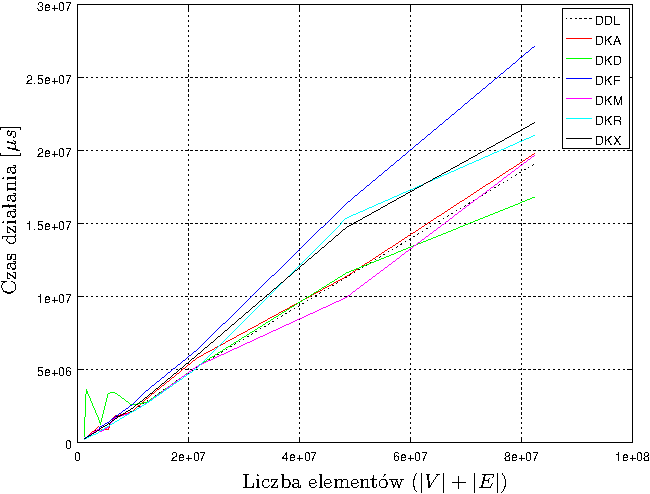
\includegraphics[width=0.72\textwidth]{Chapter_IV/USA-road-d_psfrag.pdf}
	\caption{\textbf{ Porównanie algorytmów dla testu \textsc{USA}.} Wszystkie punkty testowe zostały przedstawione w tabeli \ref{tab:USARoad}.}\label{fig:plotUSA-road-d}
\end{figure}

\begin{table}[ht]
\centering
\begin{tabular}{cccc}
\hline
\multirow{2}{*}{Skrót} & \multicolumn{2}{|c|}{Charakterystyka} & \multirow{2}{*}{Opis} \\ \cline{2-3}
& \multicolumn{1}{|c|}{Struktura} & \multicolumn{1}{c|}{Typ} &  \\
\hline
\textcolor{lgray}{\textbf{BFM}} & --- & \textsc{LCA} & Podstawowa implementacja algorytmu Bellmana-Forda \\
\textcolor{lgray}{\textbf{BFP}} & --- & \textsc{LCA} & \textsc{BFM} ze sprawdzaniem rodziców \\
\textbf{DDL} & Kubełki & \textsc{LSA} & Algorytm Dial (Dijkstra) \\
\textbf{DKA} & Kubełki & \textsc{LCA} & Algorytm z aproksymacją zakresu (Dijkstra) \\
\textcolor{lgray}{\textbf{DKB}} & Kubełki & \textsc{LSA} & Podstawowa implementacja (Dijkstra) \\
\textbf{DKD} & Kubełki & \textsc{LSA} & Algorytm dwupoziomowy (Dijkstra) \\
\textbf{DKM} & Kubełki & \textsc{LSA} & Algorytm z przepełnieniem (Dijkstra) \\
\textcolor{lgray}{\textbf{DKX}} & Kubełki & \textsc{LSA} & Podstawowa implementacja \textsf{RadixHeap} (Dijkstra) \\
\textbf{DKX} & Kubełki & \textsc{LSA} & \textsf{RadixHeap} z przepełnieniem (Dijkstra) \\
\textcolor{lgray}{\textbf{DKF}} & Kopce & \textsc{LSA} & Algorytm Dijkstry dla kopców Fibonacciego \\
\textbf{DKF} & Kopce & \textsc{LSA} & Usprawniona implementacja \text{DKF} \\
\textcolor{lgray}{\textbf{DKH}} & Drzewa & \textsc{LSA} & Algorytm Dijkstry dla $K$-drzew \\
\textbf{DKR} & Kopce & \textsc{LSA} & Implementacja algorytmu Dijkstry dla $R$-kopców \\
\textcolor{lgray}{\textbf{DKQ}} & $S$-Listy & \textsc{LSA} & Naiwny algorytm Dijkstry \\
\textcolor{lgray}{\textbf{DKQ}} & $DL$-Listy & \textsc{LSA} & Naiwny algorytm Dijkstry \\
\textcolor{lgray}{\textbf{PAP}} & Kolejki & \textsc{LSA} & Algorytm Pape'a \\
\textbf{TQQ} & Kolejki & \textsc{LSA} & Algorytm Pallottino z dwoma kolejkami \\
\textcolor{lgray}{\textbf{GR1}} & --- & \textsc{LSA} & Algorytm topologiczny \\
\textcolor{lgray}{\textbf{GR2}} & --- & \textsc{LSA} & Algorytm topologiczny z uaktualnianiem odległości \\
\textbf{THR} & $DL$-Listy & \textsc{LCA} & Algorytm progowy \\
\hline
\end{tabular}
\caption{Lista testowanych algorytmów wraz z odrzuconymi implementacjami o zbyt dużej złożoności czasowej lub pamięciowej.}
\label{tab:testAlg}
\end{table}

Pierwsze, co najbardziej rzuca się w oczy to potwierdzenie naszych słów, dotyczących algorytmu Dijkstry, który opierał się na kopcach Fibonacciego. Pomimo, że algorytm ten wydawał się najszybszy spośród wszystkich, które zostały przedstawione (poza implementacją \textsc{RadixHeap}, którego złożoność wyniosła $ O \left( m + n \cdot \log \left( C\right) \right)$), dla prawdziwych sieci drogowych, na jakich przyszło nam testować ten algorytm, działa on najwolniej ze wszystkich pozostałych, dla których wykonano te same testy. Co się okazuje, także implementacja algorytmu \textsc{RadixHeap} nie przyniosła w testach oczekiwanych rezultatów, gdyż jej szybkość działania także ustępuje większości z pozostałych algorytmów. Co natomiast się potwierdziło to stwierdzenie, zawarte w~\cite{GIDA}, jakoby najszybszymi implementacjami dla prawdziwych sieci drogowych, były algorytmy Dijkstry, wykorzystującymi kubełki aproksymacyjne (\textsc{DKA}) oraz~--- bez cienia wątpliwości~--- kubełki wielopoziomowe (\textsc{DKD}), których stopień nachylenia do poziomej osi wykresu pozwala sądzić, że wraz ze wzrostem liczby danych algorytm utrzymałby swoją dominację nad pozostałymi. Wszystkie algorytmy w trakcie testów przyjęły parametry domyślne (jeżeli takowe były wymagane tak jak np. w algorytmie \textsc{DKA})~--- optymalne, wyliczone albo przez sam algorytm, w oparciu o metody wyliczania ekstremów na podstawie wzoru, określającego rząd złożoności takiego algorytmu, albo wyliczone zawczasu, których optymalność została udowodniona). Zwrócić warto uwagę, że wszystkie dane testowe, jaki dostarczył \textsf{DIMACS Implementation Challenge}, reprezentują grafy dość rzadkie~--- sieci o większej gęstości próżno szukać w prawdziwych warunkach, chociażby ze względu na dominujące typy skrzyżowań samych dróg, gdzie w takich można wyróżnić od trzech do czterech odnóg, chyba że mamy do czynienia z większym elementem konstrukcyjnym, jakim jest rondo (co w języku grafu przekłada się na kilka węzłów, ułożonych w okręgu, od których odchodzą co najwyżej trzy krawędzie). Z tego też względu w następnym rozdziale zajmiemy się badaniem grafów o nienaturalnie~--- jak na sieci drogowe~--- dużych gęstościach, rozpoczynających się od $m = O \left( n^{1.2} \right)$, a kończących się na $m = O \left( n^{2.0} \right)$.

\section{Gęstość grafu}

W tej części eksperymentów zajmiemy się badaniem bezpośredniego wpływu gęstości grafu na zachowanie się algorytmu. Będziemy do tego korzystać z losowo wygenerowanych grafów, gdyż odnalezienie odpowiednich, rzeczywistych danych testowych byłoby niezwykle trudnym zadaniem, co uzasadniliśmy powyżej. Tak jak widzieliśmy podczas pierwszych eksperymentów, $12$ punktów kontrolnych to bardzo niewiele, a tym razem chcemy uzyskać grafy o jak najbardziej zbliżonej gęstości w znacznie większej liczbie (dla każdego zestawu grafów o zadanej gęstości będziemy chcieli mieć na tyle dużo punktów, by gęsto pokryć nimi jedną z osi wykresu, reprezentującej liczbę elementów w grafie testowym). W odróżnieniu od poprzednich testów, tym razem wykorzystamy do nich niewielkie liczby danych, za to będziemy chcieli, aby dla zadanego grafu każdy algorytm wykonał dokładnie $n$ niezależnych iteracji, gdzie $n$ to liczba węzłów w grafie.

\subsection{Metodyka i dane}

Zdając się na pseudolosowość przy generowaniu danych testowych musimy ograniczyć wpływ tego niedeterministycznego elementu na otrzymywane wyniki. Wszystkie testy otrzymujemy poprzez wygenerowanie odpowiedniej liczby wierzchołków, wyliczenie prawdopodobieństwa, z jakim powinny pojawiać się łuki w grafie dla zadanej gęstości oraz utworzenie danej liczby krawędzi, zgodnie z wcześniejszymi rachunkami. Ne mamy przy tym zagwarantowanego, że wszystkie węzły w sieci będą miały jakiekolwiek połączenie~--- im mniejsza gęstość zostanie zadana, tym to prawdopodobieństwo jest mniejsze. Może się więc zdarzyć, że ze źródła, dla którego algorytmy będą wyszukiwały najkrótsze ścieżki do wszystkich pozostałych węzłów w grafie, nie prowadzi żadna ścieżka, bądź też jest ich niewiele. Czas działania takiego algorytmu ulegnie w takim przypadku nienaturalnemu skróceniu, co oczywiście nie jest pożądane. Aby zapobiec takim sytuacjom będziemy chcieli, by dla każdego grafu $ G = \left( V, E \right) $ algorytmy wyszukiwania najkrótszych ścieżek były uruchamiane osobno dla każdego wierzchołka $v \in V$ w charakterze źródła a następnie pod uwagę była brana średnia ich czasu działania, będąca wynikiem podzielenia całkowitego czasu, jaki algorytm potrzebował na wykonanie zadania, przez liczbę wierzchołków w grafie, jakie algorytm po kolei przyjmował za węzły startowe. Przykładowe dane testowe przedstawia tabela \ref{tab:denceTest}.

\begin{table}[h]
\centering
\begin{tabular}{lcccccccc}
\hline
\multicolumn{2}{c|}{\multirow{2}{*}{Nazwa Testu}} & \multicolumn{2}{c|}{\multirow{2}{*}{Liczba elementów}} & \multicolumn{4}{c}{Budowa sieci} &  \\ \cline{5-9}
\multicolumn{2}{l|}{} & \multicolumn{2}{c|}{} & \multirow{2}{*}{Gęstość} & \multicolumn{3}{|c}{Statystyki kosztów} &  \\ \cline{1-4} \cline{6-9}
\multicolumn{1}{l|}{Numer} & \multicolumn{1}{c|}{Rząd gęstości} & \multicolumn{1}{c|}{Wierzchołków} & \multicolumn{1}{c|}{Krawędzi} & & \multicolumn{1}{|c}{$\max \left( c_{ij} \right) $} & \multicolumn{1}{|c}{$ avg \left( c_{ij} \right) $} & \multicolumn{1}{|c}{$\sigma \left( c_{ij} \right) $} &  \\
\hline
\textbf{234} & $ m = O \left( n^{1,4} \right) $ & $7~400$ & $261~170$ & $35,3$ & $1~000$ & $499,90$ & $288,76$ &  \\
\textbf{235} & $ m = O \left( n^{1,4} \right) $ & $7~500$ & $266~125$ & $35,5$ & $1~000$ & $499,60$ & $289,42$ &  \\
\textbf{236} & $ m = O \left( n^{1,4} \right) $ & $7~600$ & $271~105$ & $35,7$ & $1~000$ & $500,68$ & $289,18$ &  \\
\textbf{237} & $ m = O \left( n^{1,4} \right) $ & $7~700$ & $276~113$ & $35,9$ & $1~000$ & $500,35$ & $288,49$ &  \\
\textbf{238} & $ m = O \left( n^{1,4} \right) $ & $7~800$ & $281~146$ & $36,0$ & $1~000$ & $499,60$ & $288,78$ &  \\
\textbf{239} & $ m = O \left( n^{1,4} \right) $ & $7~900$ & $286~205$ & $36,2$ & $1~000$ & $503,14$ & $288,74$ &  \\
\textbf{240} & $ m = O \left( n^{1,4} \right) $ & $8~000$ & $291~290$ & $36,4$ & $1~000$ & $499,90$ & $288,78$ &  \\
\textbf{...} & $ \cdots $ & $ \cdots $ & $ \cdots $ & $ \cdots $ & $ \cdots $ & $ \cdots $ & $ \cdots $ &  \\
\textbf{474} & $ m = O \left( n^{1,8} \right) $ & $7~400$ & $9~217~583$ & $1245,6$ & $1~000$ & $500,03$ & $288,68$ &  \\
\textbf{475} & $ m = O \left( n^{1,8} \right) $ & $7~500$ & $9~443~006$ & $1259,1$ & $1~000$ & $499,95$ & $289,05$ &  \\
\textbf{476} & $ m = O \left( n^{1,8} \right) $ & $7~600$ & $9~670~845$ & $1272,5$ & $1~000$ & $499,89$ & $289,23$ &  \\
\textbf{477} & $ m = O \left( n^{1,8} \right) $ & $7~700$ & $9~901~096$ & $1285,9$ & $1~000$ & $502,13$ & $288,89$ &  \\
\textbf{478} & $ m = O \left( n^{1,8} \right) $ & $7~800$ & $10~133~752$ & $1299,2$ & $1~000$ & $500,52$ & $289,38$ &  \\
\textbf{479} & $ m = O \left( n^{1,8} \right) $ & $7~900$ & $10~368~806$ & $1312,5$ & $1~000$ & $499,77$ & $288,77$ &  \\
\textbf{480} & $ m = O \left( n^{1,8} \right) $ & $8~000$ & $10~606~252$ & $1325,9$ & $1~000$ & $501,64$ & $288,73$ &  \\
\hline
\end{tabular}
\caption{Dane testowe dla różnych gęstości sieci}
\label{tab:denceTest}
\end{table}

Możemy wyróżnić $6$ poziomów gęstości grafu, dla których w tym podrozdziale zostały przeprowadzone eksperymenty, gdzie dla każdego z nich liczba krawędzi w grafie jest rzędu $ O \left( n^{2.0-i \cdot 0.2} \right)$ dla $i \in \left\{ 0, \cdots, 5 \right\}$, zaś każdy z nich składa się z $80$ grafów, charakteryzujących się stopniowo zwiększaną liczbą wierzchołków. Co oczywiste - w powyższej tabeli nie przedstawiono wszystkich danych testowych, gdyż łącznie jest ich ponad $450$, zaś zasada ich konstrukcji~--- taka sama. Dane te zostały wygenerowane bezpośrednio na serwerze, aby uniknąć konieczności ich wysyłania. Każdy z algorytmów, dla którego zostały przeprowadzone powyższe testy, był uruchamiany równolegle wraz z pozostałymi algorytmami, wykorzystując moc obliczeniową serwera~--- czas, w jakim była mierzona efektywność algorytmów jest czasem, jakie algorytmy łącznie dostały od któregoś z procesorów na wykonywanie zadań, więc takie postępowanie (równoległe uruchomienie testów) nie miało wpływu na otrzymane wyniki. Tym samym w czas trwania algorytmów nie został w pełni poprawnie wliczony czas, jaki każdy z nich potrzebował na wczytanie danych i stworzenie własnych struktur, których~--- jak pokazaliśmy dobitnie w części teoretycznej~--- prawie każdy potrzebuje, a które znacznie potrafią różnić się od siebie wymaganiami i czasem ich tworzenia (np. algorytm oparty na kopcach nie potrzebował tego czasu prawie w ogóle, gdyż do pracy wymagał tworzenia tylko paru pomocniczych zmiennych). Zwłaszcza samo wczytanie danych przez algorytmy zostało pominięte~--- składały się na nie operacje wejścia/wyjścia, które nie są liczone jako czas efektywnie wykorzystywany przez procesor. Aby uwzględnić i tę część działania każdej z implementacji, należałoby powołać się na rzeczywisty upływ czasu~--- wtedy jednak uruchomienie kilku algorytmów równolegle byłoby niedopuszczalne. Poniżej przedstawiono wykresy zależności, jakie zostały otrzymane dla grafów o różnym stopniu gęstości (wykresy: \ref{fig:plotFullGraph_1.20}, \ref{fig:plotFullGraph_1.40}, \ref{fig:plotFullGraph_1.60}, \ref{fig:plotFullGraph_1.80} i \ref{fig:plotFullGraph_2.00}) a na których możemy zaobserwować jaki ogromny wpływ na efektywność poszczególnych algorytmów ma ich gęstość. Z całą stanowczością należy jeszcze raz podkreślić, że przedstawione poniżej wykresy dotyczą sieci, których gęstość jest nienaturalnie wysoka w odniesieniu do rzeczywistych sieci drogowych a przedstawienie tych wyników eksperymentalnych ma na celu ukazać różne sposoby zachowania się algorytmów ze względu na ten parametr.

\subsection{Wyniki i wykresy zależności}

Charakterystycznym elementem wybranych sieci, które zostały przedstawione w tabeli \ref{tab:denceTest}, jest ich nienaturalna regularność~--- dla gęstości rzędu $ m = O \left( n^{1+\epsilon}\right)$, gdzie $ 0,2 \leqslant \epsilon \leqslant 1.0 $ liczba krawędzi dla każdego z wierzchołków jest pomniejszana (w stosunku do grafu, gdzie  $ m = O \left( n^{2}\right)$) równomiernie w odniesieniu do pozostałych węzłów w sieci. Daje to w wyniku graf, który nie posiada żadnych wyraźniejszych skupisk elementów~--- jego gęstość pozostaje taka sama, bez względu na to, na który fragment grafu spojrzymy.

\begin{figure}[!htbp]
	\centering
	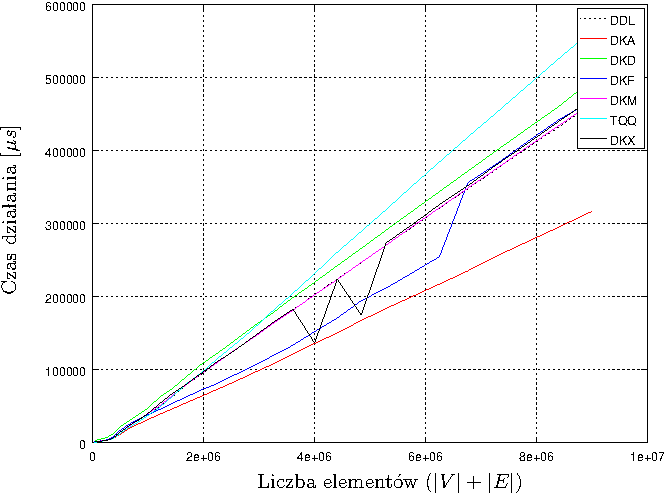
\includegraphics[width=0.85\textwidth]{Chapter_IV/fullGraph200_psfrag.pdf}
	\caption{\textbf{ Porównanie algorytmów dla grafu o gęstości, wyrażonej równością $ m = O \left( n^{2} \right)$.} Na osi poziomej wykresu przedstawiona jest suma liczby wierzchołków oraz krawędzi w grafie. Oś \textsc{OY} przedstawia ilość czasu w mikrosekundach ($\mu = 10^{-6} s$). }\label{fig:plotFullGraph_2.00}
\end{figure}

\begin{figure}[!htbp]
	\centering
	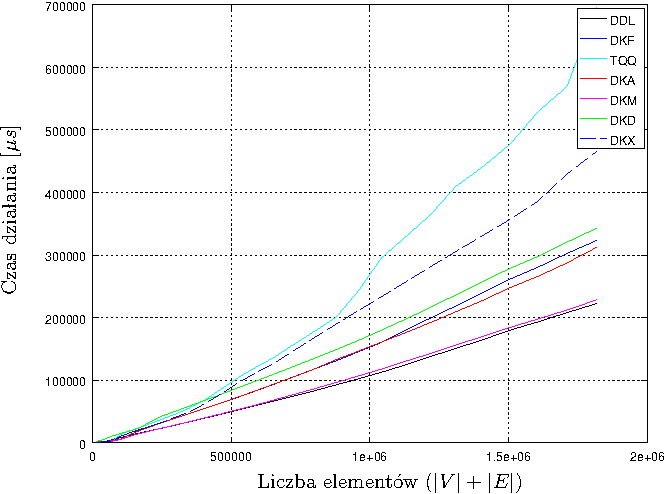
\includegraphics[width=0.85\textwidth]{Chapter_IV/graph180_psfrag.pdf}
	\caption{\textbf{ Porównanie algorytmów dla grafu o gęstości, wyrażonej równością $ m = O \left( n^{1.8} \right)$.}}\label{fig:plotFullGraph_1.80}
\end{figure}

\begin{figure}[!htbp]
	\centering
	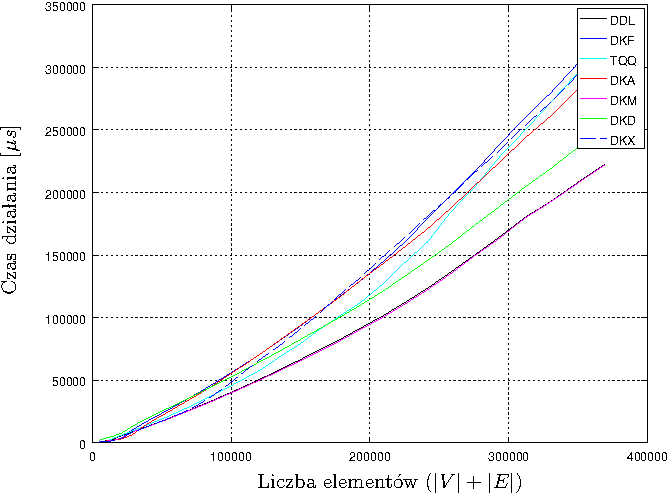
\includegraphics[width=0.85\textwidth]{Chapter_IV/graph160_psfrag.pdf}
	\caption{\textbf{ Porównanie algorytmów dla grafu o gęstości, wyrażonej równością $ m = O \left( n^{1.6} \right)$.}}\label{fig:plotFullGraph_1.60}
\end{figure}

\begin{figure}[!htbp]
	\centering
	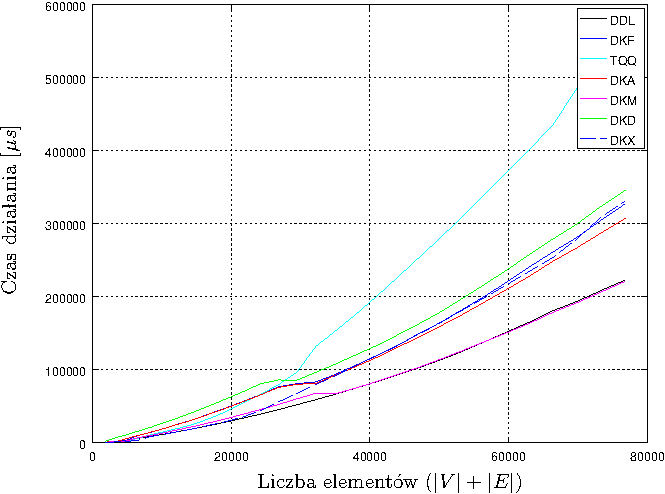
\includegraphics[width=0.85\textwidth]{Chapter_IV/graph140_psfrag.pdf}
	\caption{\textbf{ Porównanie algorytmów dla grafu o gęstości, wyrażonej równością $ m = O \left( n^{1.4} \right)$.}}\label{fig:plotFullGraph_1.40}
\end{figure}

\begin{figure}[!htbp]
	\centering
	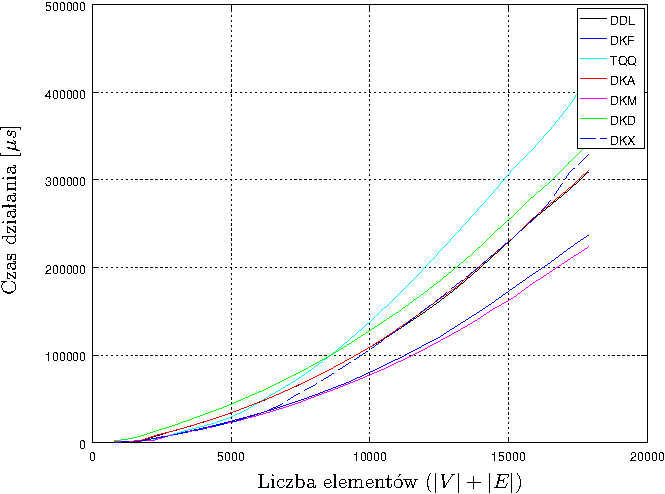
\includegraphics[width=0.85\textwidth]{Chapter_IV/graph120_psfrag.pdf}
	\caption{\textbf{ Porównanie algorytmów dla grafu o gęstości, wyrażonej równością $ m = O \left( n^{1.2} \right)$.}}\label{fig:plotFullGraph_1.20}
\end{figure}

\newpage

\section{Pozostałe testy}

Uważny czytelnik mógł z pewnością zauważyć, że wyliczone zależności pomiędzy czasem działań poszczególnych algorytmów w najgorszych przypadkach nie do końca pokrywają się z przedstawionymi wynikami. W szczególności na uwagę zasługują implementacje i ich złożoności, które przedstawione są w tabeli \ref{tab:wcaSummary}

\begin{table}[!htbp]
	\centering
	\begin{tabular}{ccc}
		Algorytm & Analiza \textsc{WCA} \\
		\hline \\
		\textbf{DKA} & $ O \left( m \cdot b + n \cdot \left( b + \frac{C}{b}\right)\right)$ \\
		\textbf{DKF} & $ O \left( m + n \cdot \log \left( n \right) \right)$ \\
		\textbf{DKX} & $O \left( m + n \cdot \log \left( C \right) \right)$ \\
		\textbf{DDL} & $O \left( m + n \cdot C  \right)$ \\
		\textbf{DKD} & $O \left( m + n \cdot \sqrt{C} \right)$ \\
		\hline
	\end{tabular}
	\caption{\textbf{Podsumowanie najważniejszych złożoności algorytmów}, silnie zależnych od parametru $C$ (przypominamy, że $ C = \max \left\{ c_{ij} : e_{ij} \in E \right\}$).}
	\label{tab:wcaSummary}
\end{table}

\subsection{Metodyka i dane}

Przedstawione algorytmy zostały przetestowane przy wykorzystaniu sieci, których użyliśmy w pierwszej części eksperymentów, a które przedstawiliśmy w tabeli \ref{tab:USARoad}. Jedynymi modyfikacjami jakich się dopuścimy wobec wspomnianych sieci były zmiany parametrów $c_{ij}$ związanych z każdą krawędzią $v_{i} \overset{1} \leadsto v_{j}$~--- odpowiednio zostały one przemnożone przez następujące stałe: $10$, $50$ i $100$. Testy przeprowadzono tak samo jak we wcześniej wspomnianych eksperymentach, gdzie wykorzystywaliśmy grafy przedstawiające sieć dróg Stanów Zjednoczonych Ameryki~--- dla każdego z punktów testowych algorytmy zostały uruchomione $t = 40$ razy, przy czym dla każdego takiego punktu algorytm miał za zadanie wyszukać wszystkie najkrótsze ścieżki ze źródeł, które z góry zostały ustalone. Dla każdego z testów wybrano równo $500$ takich źródeł.

\subsection{Wyniki i wykresy zależności}

\begin{figure}[!htbp]
	\centering
	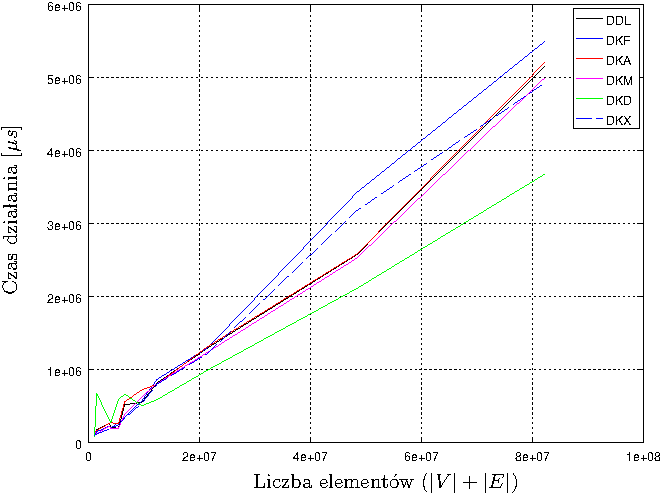
\includegraphics[width=0.65\textwidth]{Chapter_IV/graphx1Cost_psfrag.pdf}
	\caption{ \textbf{Porównanie algorytmów dla testu \textsc{USA}} ze zwiększonymi kosztami ($\forall e_{ij} \in E \: : \: c^{'}_{ij} = c_{ij} \cdot 10$).}\label{fig:plotgraphx10Cost}
\end{figure}

\begin{figure}[!htbp]
	\centering
	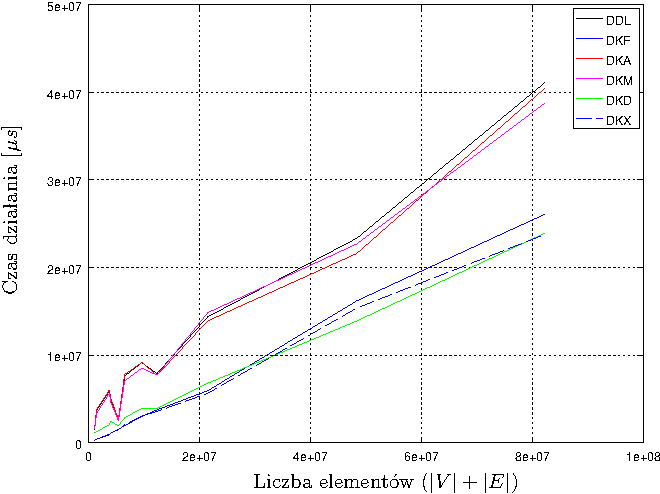
\includegraphics[width=0.82\textwidth]{Chapter_IV/graphx10Cost_psfrag.pdf}
	\caption{\textbf{\textbf{Porównanie algorytmów dla testu \textsc{USA}} ze zwiększonymi kosztami ($\forall e_{ij} \in E \: : \: c^{'}_{ij} = c_{ij} \cdot 50$).} Wszystkie punkty testowe zostały przedstawione w tabeli \ref{tab:USARoad}.} \label{fig:plotgraphx50Cost}
\end{figure}
\begin{figure}[!htbp]
	\centering
	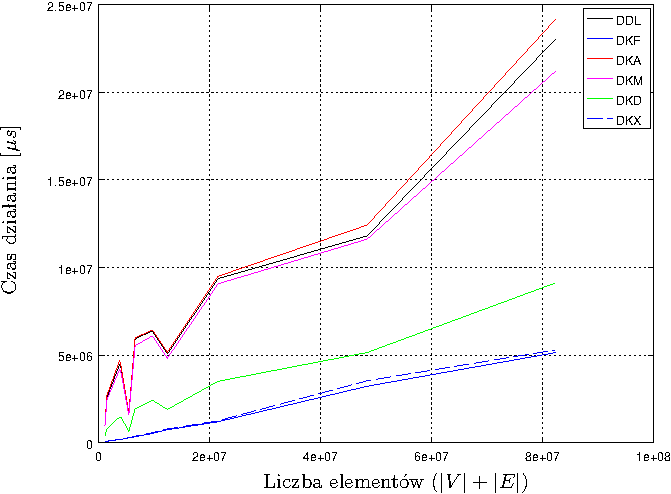
\includegraphics[width=0.82\textwidth]{Chapter_IV/graphx50Cost_psfrag.pdf}
	\caption{\textbf{\textbf{Porównanie algorytmów dla testu \textsc{USA}} ze zwiększonymi kosztami ($\forall e_{ij} \in E \: : \: c^{'}_{ij} = c_{ij} \cdot 100$).} Wszystkie punkty testowe zostały przedstawione w tabeli \ref{tab:USARoad}.} \label{fig:plotgraphx100Cost}
\end{figure}

W oparciu o wyniki, przedstawione na wykresach \ref{fig:plotgraphx10Cost}, \ref{fig:plotgraphx50Cost} oraz \ref{fig:plotgraphx100Cost}, możemy ponad wszelką wątpliwość wskazać algorytmy, których złożoność obliczeniowa w znacznej mierze zależy od parametru $C$. Jeżeli spojrzymy jeszcze raz na dane w tabeli \ref{tab:wcaSummary}, zobaczymy że wraz z rosnącymi kosztami w grafie rośnie przepaść między dwoma grupami algorytmów, gdzie w jednej z nich znajdują się algorytmy takie jak: \textsc{DKF}, \textsc{DKX} oraz \textsc{DKD}. Jak dobrze pamiętamy, algorytm Dijkstry, zbudowany w oparciu o kopce Fibonacciego, był jednym z wolniejszych algorytmów, jakie testowaliśmy. Wraz z rosnącymi kosztami w grafie sytuacja się odwraca i staje się on jednym z najszybszych. Przyczyną tego typu zachowania jest oczywiście brak zależności między nim a rosnącymi kosztami każdej z krawędzi ($ O \left( m + n \cdot \log \left( n \right) \right)$). Pozostałe algorytmy zależne od $C$ mają nałożoną na tę zmienną funkcję, która w znaczny sposób niweluje wpływ zwiększania się jej na efektywność danej implementacji (odpowiednio dla \textsc{DKX} i \textsc{DKD} są to: $\log \left( C \right)$ oraz $ \sqrt[2]{C}$). Nie zaprezentowaliśmy tutaj złożoności algorytmu \textsc{DKM}, gdyż jego złożoność ograniczyliśmy przez $O \left( n^{2} \right)$. Jak jednak łatwo było zauważyć w czasie jej analizy (\ref{DKMComplexity}), takie oszacowanie głównie wynikało z konieczności wyszukiwania minimalnego elementu z ostatniego kubełka w algorytmie dla każdej z rund. Przyglądając się dokładniej wspomnianej analizie łatwo zauważyć, że i ten algorytm wykazuje się silną zależnością od maksymalnego kosztu w sieci ($O \left( n \cdot C \right)$), podobnie z resztą jak algorytm Dial oraz \textsc{DKA} ($O \left( n \cdot C \cdot \frac{1}{b} \right)$).

Wspominaliśmy na początku rozdziału poświęconego eksperymentom, że implementacje wszystkich algorytmów w miarę możliwości starają się dobrać optymalne parametry dla każdego z nich, jeżeli takowe są przez dany algorytm wymagane. Nie wszystkie jednak parametry da się jednoznacznie wyliczyć, czego najlepszym przykładem jest algorytm \text{DKA}. Poniżej przedstawiono wykres zależności między dobranym parametrem dla wspomnianego algorytmu a czasem jego działania. W charakterze danych testowych ponownie zostały wykorzystane grafy, których opis znajduje się w tabeli \ref{tab:USARoad}, wielokrotnie już przywoływanej.

\begin{figure}[!htbp]
	\centering
	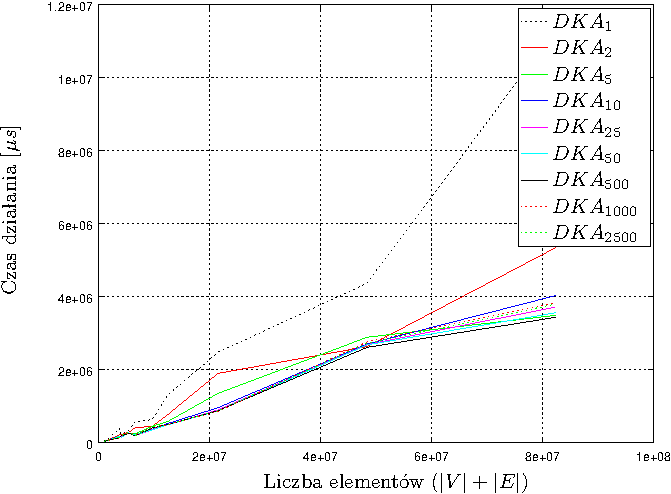
\includegraphics[width=0.9\textwidth]{Chapter_IV/DKA-param_psfrag.pdf}
	\caption{\textbf{Zależność efektywności algorytmu \textsc{DKA} od dobranego parametru}, wymaganego przez algorytm. }\label{fig:plotDKA-param}
\end{figure}

Przedstawione wyniki wyraźnie sugerują zależność między rozmiarami sieci a odpowiednio dobranym współczynnikiem, który może się okazać nieodpowiedni, jeżeli te pierwsze będą za duże, bądź za małe~\cite[$3.3.2$,$3.10.3$]{Dissertation}.